% ---------------------------------------------------------------------------- %
\section{Technical issues}
\label{ch:linguometer:technical}
% ---------------------------------------------------------------------------- %


% ---------------------------------------------------------------------------- %
\subsection{Synchronization and segmentation signals}
\label{sec:linguometer:technical:signals}
% ---------------------------------------------------------------------------- %
This section aims to discuss the properties of the synchronization and
segmentation signals. 
In the previous Section (\S\ref{sec:linguometer:architecture:diagram}), the
linguometer workflow diagram has been described. 
Furthermore, it has been stressed the fact that the synchronization of the 
ultrasonograpic and the articulographic data strictly depends onto the 
\wf{US-DV} stream.

Figure~\ref{fig:linguometer:architecture:workflow} shows a symbolic
representation of the data \wf{US-DV} stream; 
a total of ten time-labels are used to highlight the time instants that play a
crucial role int the synchronization mechanism. 
Eight out of the ten labels are linked with a particular
synchronization/segmentation signal.

On the other hand, Figure~\ref{fig:linguometer:architecture:sig:usdv} shows a 
real example of the \wf{US-DV} track albeit the signals strictly 
resembles what already
discussed in \S\ref{sec:linguometer:architecture:diagram} (a batch of two words
is used) (?on the other hand/albeit?).
The upper plot refers to the left audio channel and shows the \wf{US-Sync}
signal. Two peaks are visible: the first one reaches the negative saturation
value (\tstart{AG}) while the latter one reaches the positive saturation value 
(\tstop{AG}).
% ---------------------------------------------------------------------------- %
\begin{figure}[!ht]
\centering
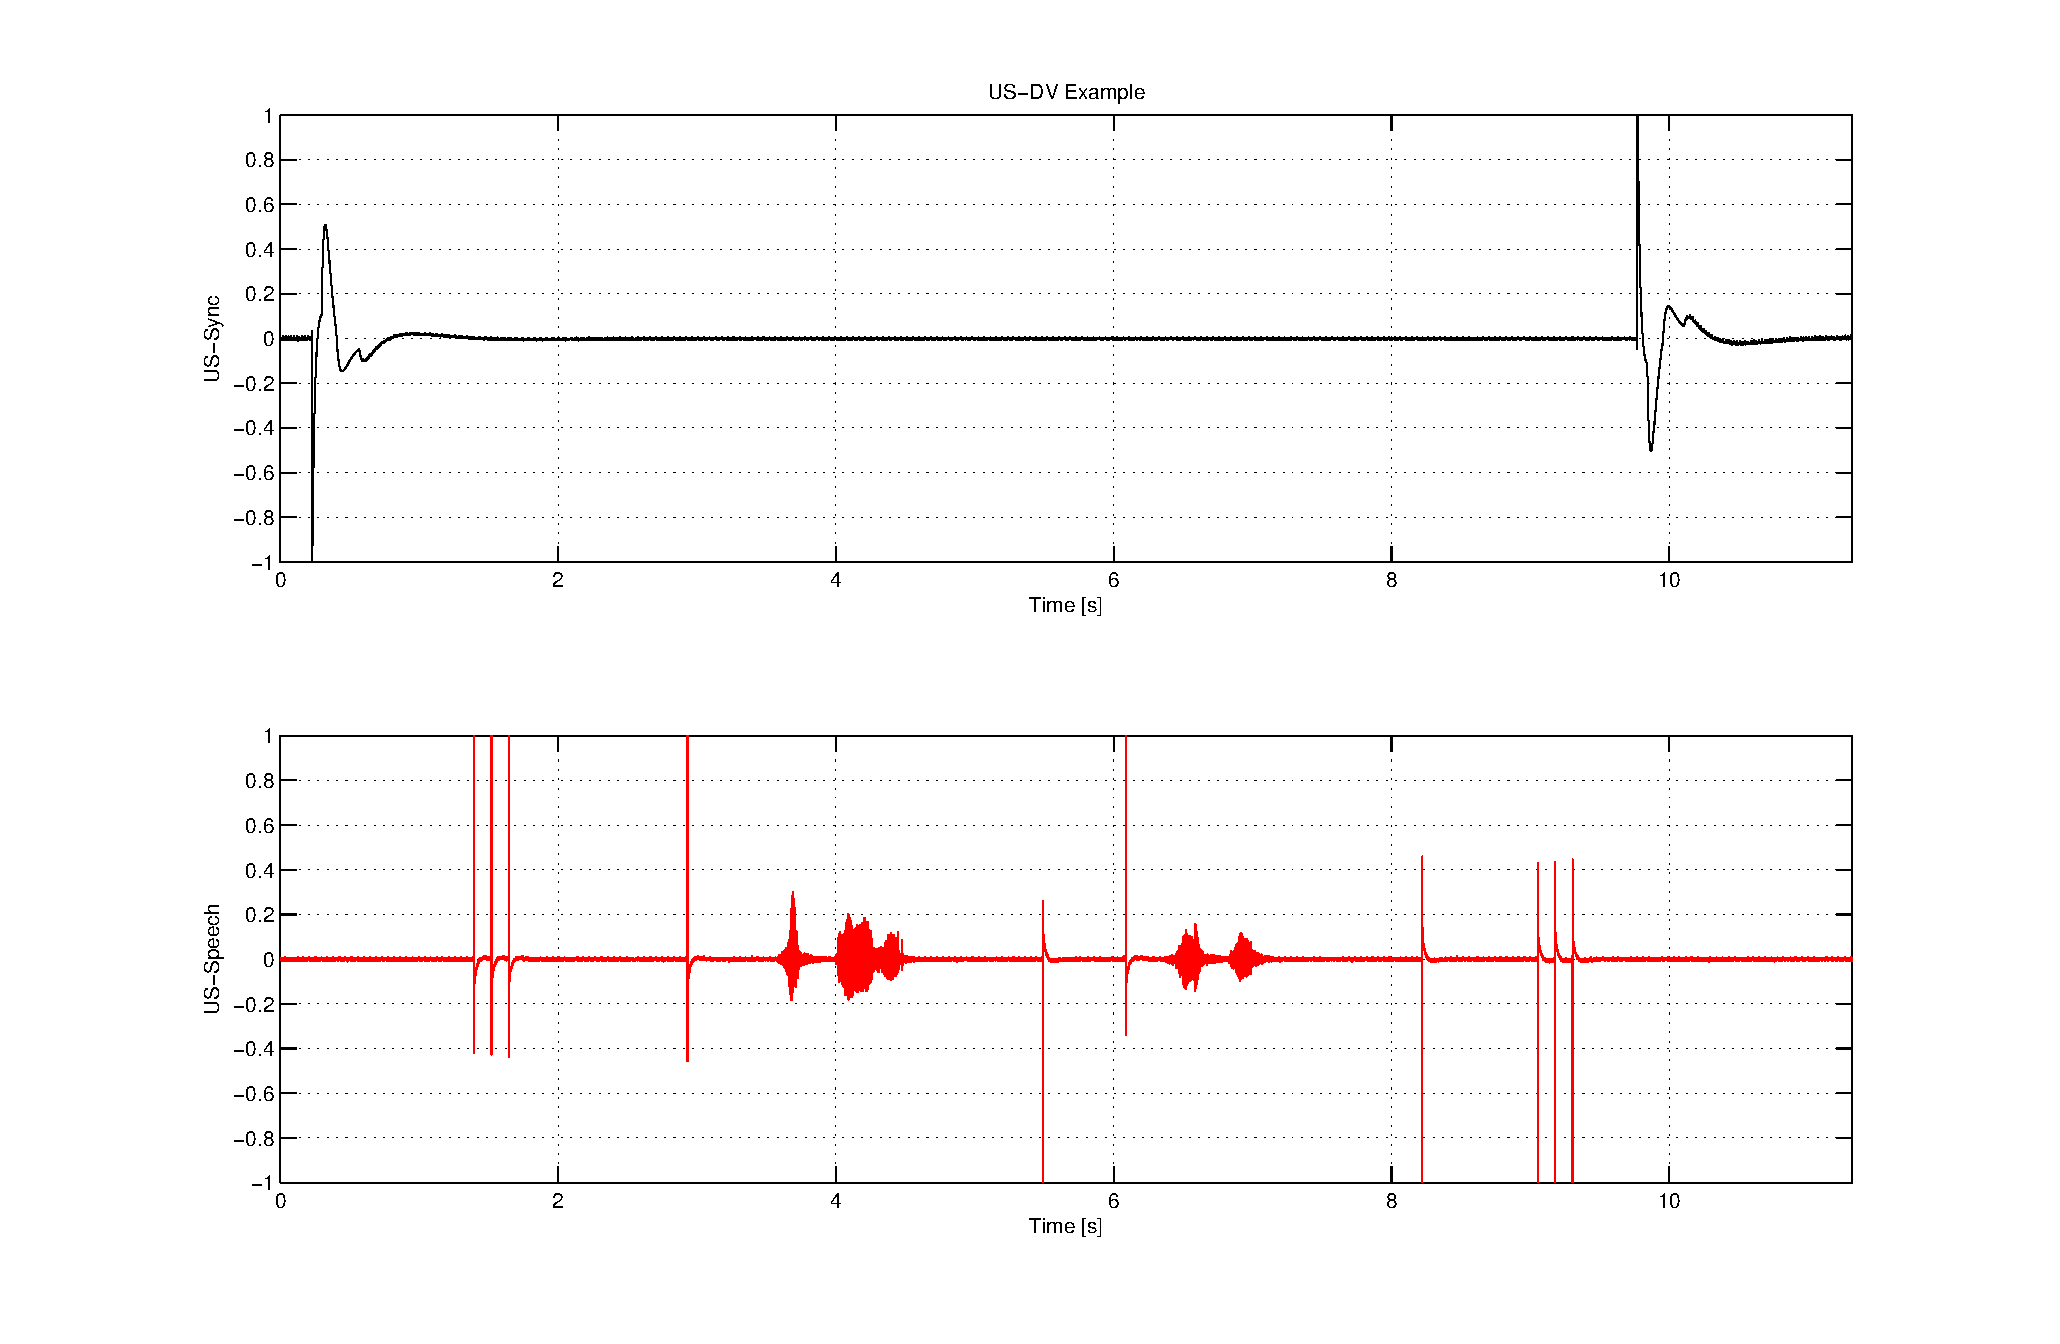
\epsfig{file=include/linguometer/images/usdv_example.eps,width=1.00\textwidth}
	\caption[US-DV Example]{\textbf{US-DV Example}: 
	(a) \wf{US-Sync} and (b) \wf{US-Speech} signals.}
	\label{fig:linguometer:architecture:sig:usdv}
\end{figure}
% ---------------------------------------------------------------------------- %

In the lower plot the \wf{US-Speech} signal is shown. This signal contains two
  main components: the speech signal itself and the segmentation signals.
A total of ten peaks are shown.
The first three peaks reach the positive saturation value and the distance
between each other is constant. 
Those peaks constitute the \emph{word batch start} signal.
Similarly, at the very end of the track, the \emph{word batch stop} signal is
shown (the cluster of three peaks that reach the negative saturation value).

The remaining four peaks constitute the \emph{word start/stop} segmentation
signals.
The first word\footnote{First word: /mattone/, /brick/ in English.}
is delimited by the fourth and the fifth peak
(\tstarti{WD}{0}, and \tstopi{WD}{0})
while the latter one\footnote{Second word: /goffo/, /clumsy/ in English.}
is delimited by the sixth and the seventh peak 
(\tstarti{WD}{1}, and \tstopi{WD}{1}).
As already discussed, the segmentation signals are generated by the
\emph{lmwords} stimuli presentation program, here described in detail.
% ---------------------------------------------------------------------------- %
\subsection{Stimuli presentation program: \emph{lmwords}}
\label{sec:linguometer:technical:lmwords}
% ---------------------------------------------------------------------------- %
\emph{lmwords} is written in C++ on and relies on the \emph{SDL} library (Simple
DirectMedia Layer)\footnote{libsdl v.1.2.11-r2, http://www.libsdl.org/.} 
for stimuli presentation and segmentation signal generation.
Providing a straightforward interface and a comprehensive set of plug-ins, 
SDL appeared as the best choice.
\emph{lmwords} instantiates a full-screen black window in which the stimuli are
rendered using the \emph{sdl-ttf} library (SDL TrueType Fonts)\footnote{sdl-ttf 
v.2.0.8 http://www.libsdl.org/projects/SDL\_ttf/.}.
The stimuli-presentation window is shown on a secondary monitor piloted by
\sig{PC0}. The segmentation signals have been created ad-hoc using the \emph{lmtools} FFMPEG interface\footnote{ffmpeg v.0.4.9, http://ffmpeg.org/.}.
% ---------------------------------------------------------------------------- %
\begin{figure}
	\centering
	\subfigure[\label{fig:linguometer:architecture:sig:lmwords2:1}]
	{\includegraphics[width=0.25\textwidth]{include/linguometer/images/lmwords_1.tps}}
	\hspace{0.05\textwidth}
	\subfigure[\label{fig:linguometer:architecture:sig:lmwords2:2}]
	{\includegraphics[width=0.25\textwidth]{include/linguometer/images/lmwords_2.tps}}
	\hspace{0.05\textwidth}
	\subfigure[\label{fig:linguometer:architecture:sig:lmwords2:3}]
	{\includegraphics[width=0.25\textwidth]{include/linguometer/images/lmwords_3.tps}}

	\subfigure[\label{fig:linguometer:architecture:sig:lmwords2:4}]
	{\includegraphics[width=0.25\textwidth]{include/linguometer/images/lmwords_4.tps}}
	\hspace{0.05\textwidth}
	\subfigure[\label{fig:linguometer:architecture:sig:lmwords2:5}]
	{\includegraphics[width=0.25\textwidth]{include/linguometer/images/lmwords_5.tps}}
	\hspace{0.05\textwidth}
	\subfigure[\label{fig:linguometer:architecture:sig:lmwords2:6}]
	{\includegraphics[width=0.25\textwidth]{include/linguometer/images/lmwords_6.tps}}
	
	\caption[Stimuli-presentation program states]{\textbf{Stimuli-presentation 
	program states}: \emph{lmwords} passes through four distinct states: (a)
	\emph{pause}, (b) \emph{ready}, (c,d) \emph{word presentation} and
	(e) \emph{done}. The last panel (f) shows how the stimuli are presented on 
	the LCD screen used during the recording sessions.
	During each state-transition, the screen remains black for half a second.
	Furthermore, the subjects are aware of meaning of each state. 
	In fact, the subjects can freely talk to the experimenters until the program
	enters in the ``pause'' state and after the program enters the ``end''
	state.}
	\label{fig:linguometer:architecture:sig:lmwords}
\end{figure}
% ---------------------------------------------------------------------------- %

Those signals are loaded and played by \emph{lmwords} using the \emph{sdl-mixer}
library\footnote{sdl-mixer v.1.2.7, http://www.libsdl.org/projects/SDL\_mixer/.}.
The \emph{lmwords} program has four main states: \emph{pause}, \emph{ready},
\emph{word presentation} and \emph{done}.
After it has been launched, \emph{lmwords} loads a batch of stimuli and mixes it
randomly, although the seed that is used to generate the normal distribution has
been kept fixed during the linguometer experiments.
The first state entered by the program is ``pause''. By pressing a key on
the \sig{PC0} keyboard, the experimenter generates the \emph{word batch start}
segmentation signal and the program enters the ``ready'' state, waiting for
user input.

% ---------------------------------------------------------------------------- %
\begin{figure}
	\centering
	\subfigure[\label{fig:linguometer:architecture:sig:lmwords:1}]
	{\includegraphics[width=\textwidth]{include/linguometer/images/seg_batch.eps}}
	
	\subfigure[\label{fig:linguometer:architecture:sig:lmwords:2}]
	{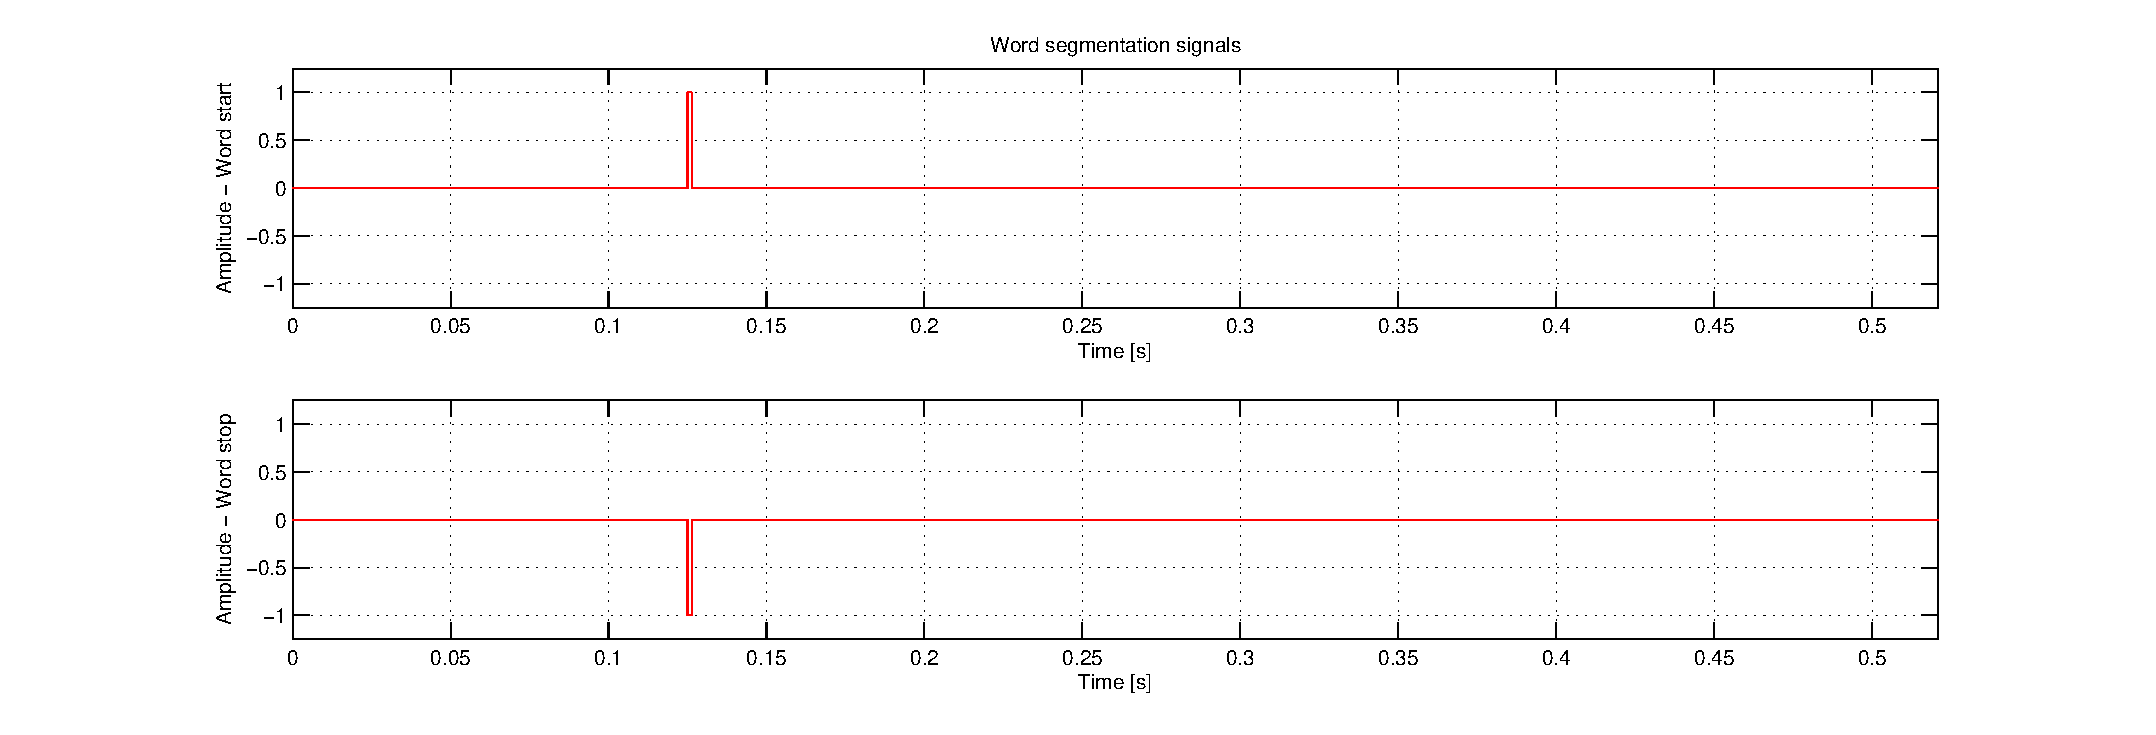
\includegraphics[width=\textwidth]{include/linguometer/images/seg_word.eps}}
	
	\caption[Segmentation signals]{\textbf{Segmentation signals}:
	the right channel component of the segmentation signals is shown (the left 
	channel has zero amplitude):
	(a) \emph{word batch start/stop} and (b) \emph{word start/stop}.
	The duration of the signals is 520 ms, while the duration of
	the peaks is 1.33 ms (64 samples). The first peak appears after 124 ms from
	the beginning of the tracks.
	In (a) the delay between two contiguous peaks is set to 124 ms. 
	Note: the amplitude axis interval is set to $[-1.50, 1.50]$ although
	the negative and positive saturation values are set to $-1.00$ and $1.00$
	respectively.
	The signals are stored in a Microsoft WAV container (PMC 16bit, 48kHz).
	}
	\label{fig:linguometer:architecture:sig:segmentation}
\end{figure}
% ---------------------------------------------------------------------------- %

Another key press causes \emph{lmwords} to enter the ``word presentation''
state: the \emph{word start} signal is generated and the first word is 
rendered on the screen.
The program remains into this latest state until the experimenter has decided if
the presented stimuli have been pronounced correctly by the subject.
The experimenter, by pressing a key, can mark the word as ``correctly
pronounced'' or ``not correctly pronounced''. 
In both cases, \emph{lmwords} generates the \emph{word stop} signal and 
moves to the next stimulus.
In the case that the word is not correctly pronounced, \emph{lmwords} queues
the stimulus so it will be presented at the end of the batch.
Once the whole set of stimuli has been presented and the whole pronounced words
have been marked as ``correctly pronounced'' by the experimenter,
\emph{lmwords} enters generates the \emph{word batch stop} signal and enters 
the ``done'' state.
Figure~\ref{fig:linguometer:architecture:sig:lmwords} shows the four
states entered by \emph{lmwords} while 
in Figure~\ref{fig:linguometer:architecture:sig:segmentation} the segmentation
signals are shown.
% ---------------------------------------------------------------------------- %
\subsection{Acquisition card and audio mixer delay}
\label{sec:linguometer:technical:delay}
% ---------------------------------------------------------------------------- %
The time delays that affects both the acquisition card and the 
audio mixer have been measured.
As already discussed in this chapter, those two devices are the core of the
articulographic/ultrasonograpic data hardware synchronization mechanism.
Although the values of the measured delays appear small, knowing them is surely
useful for what regards the post-processing alignment task.
% ---------------------------------------------------------------------------- %
\begin{figure}
	\centering
	\subfigure[\label{fig:linguometer:architecture:sig:delay:7}]
	{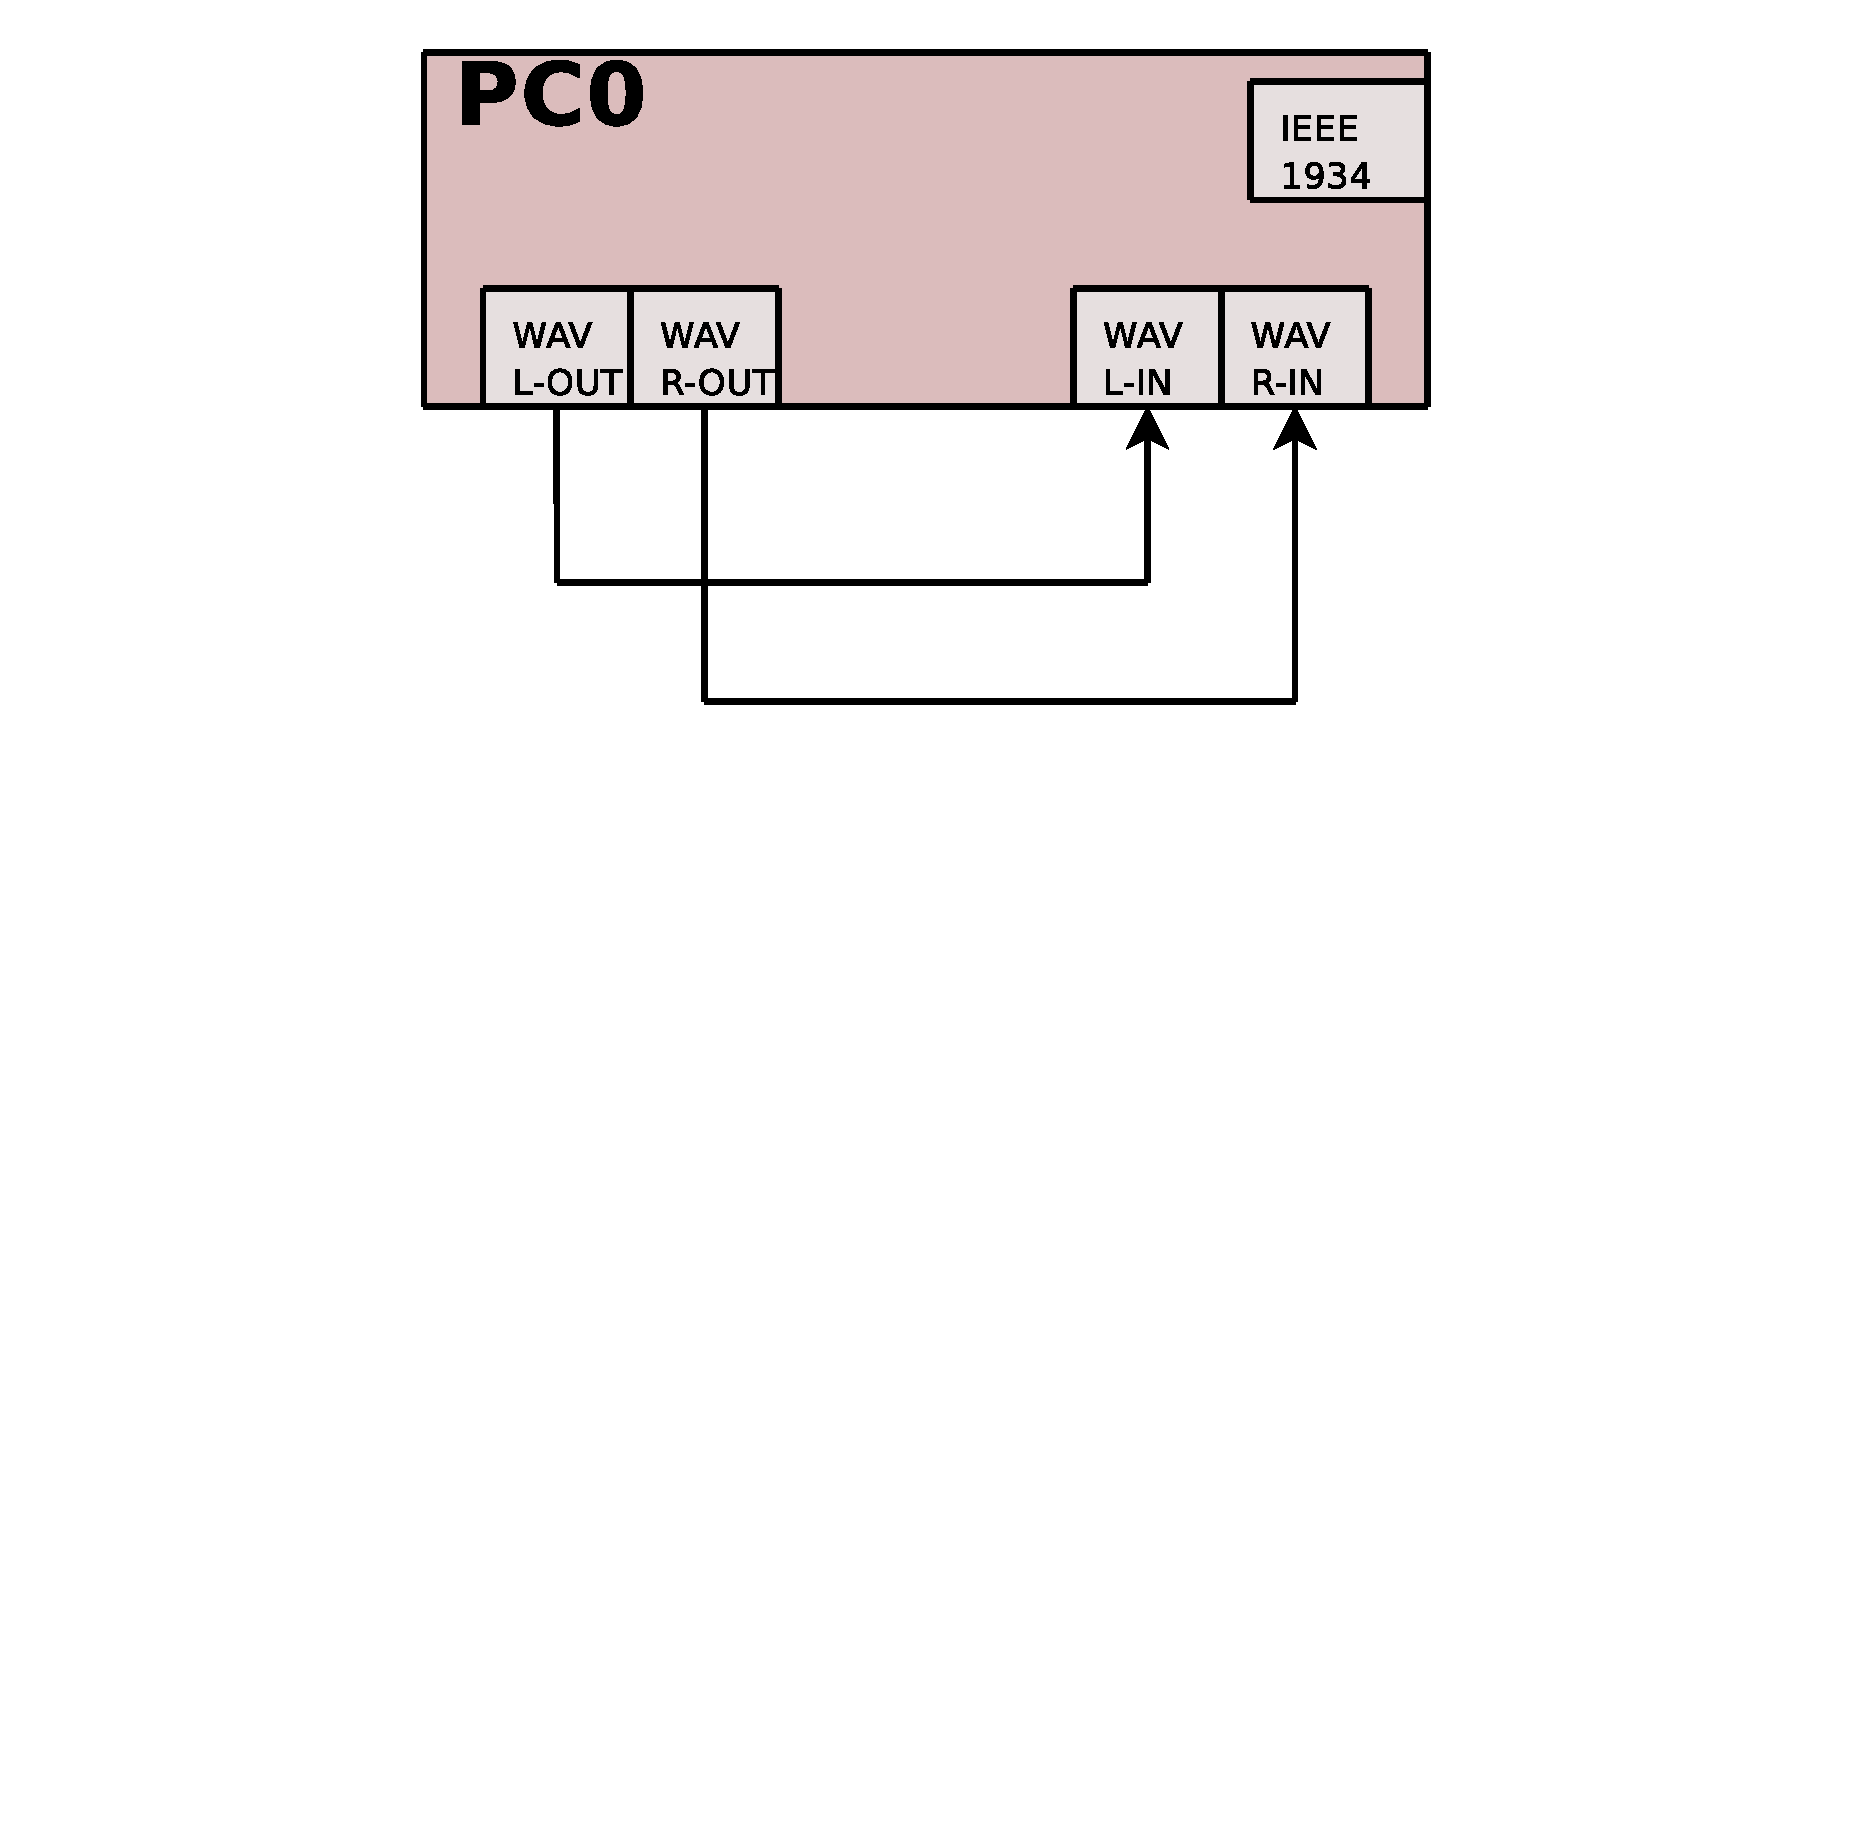
\includegraphics[width=0.32\textwidth]{include/linguometer/images/delay_schemaT.eps}}
	\subfigure[\label{fig:linguometer:architecture:sig:delay:8}]
	{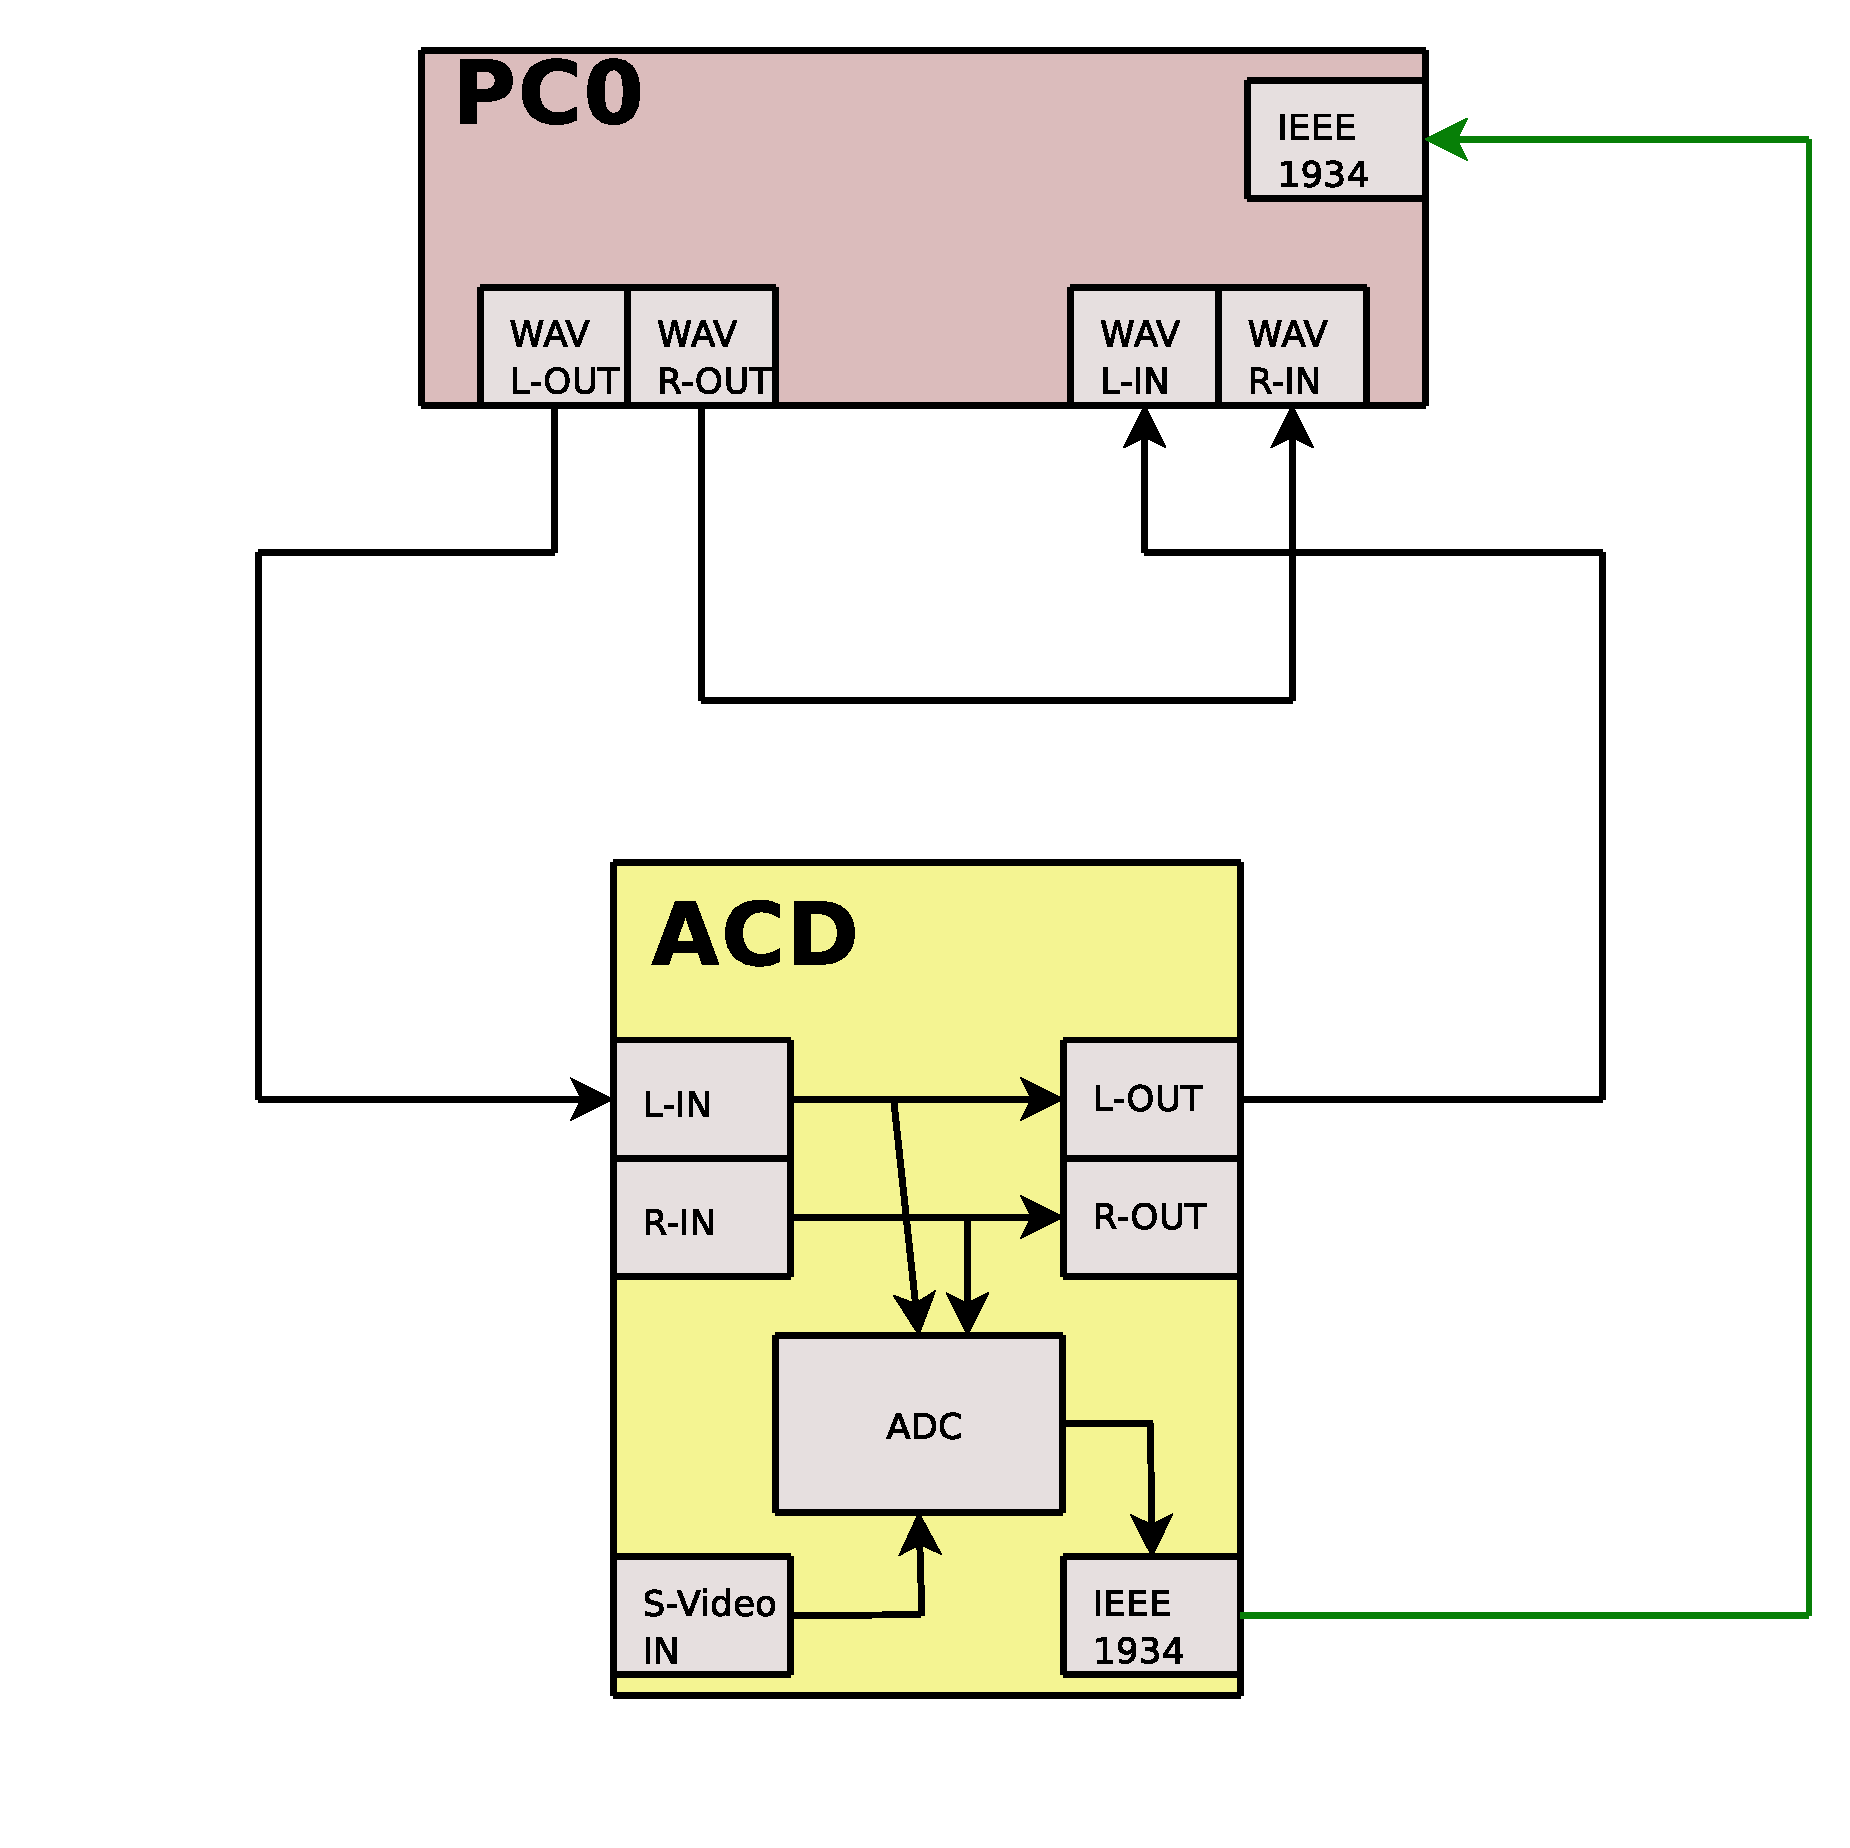
\includegraphics[width=0.32\textwidth]{include/linguometer/images/delay_schemaL.eps}}
	\subfigure[\label{fig:linguometer:architecture:sig:delay:9}]
	{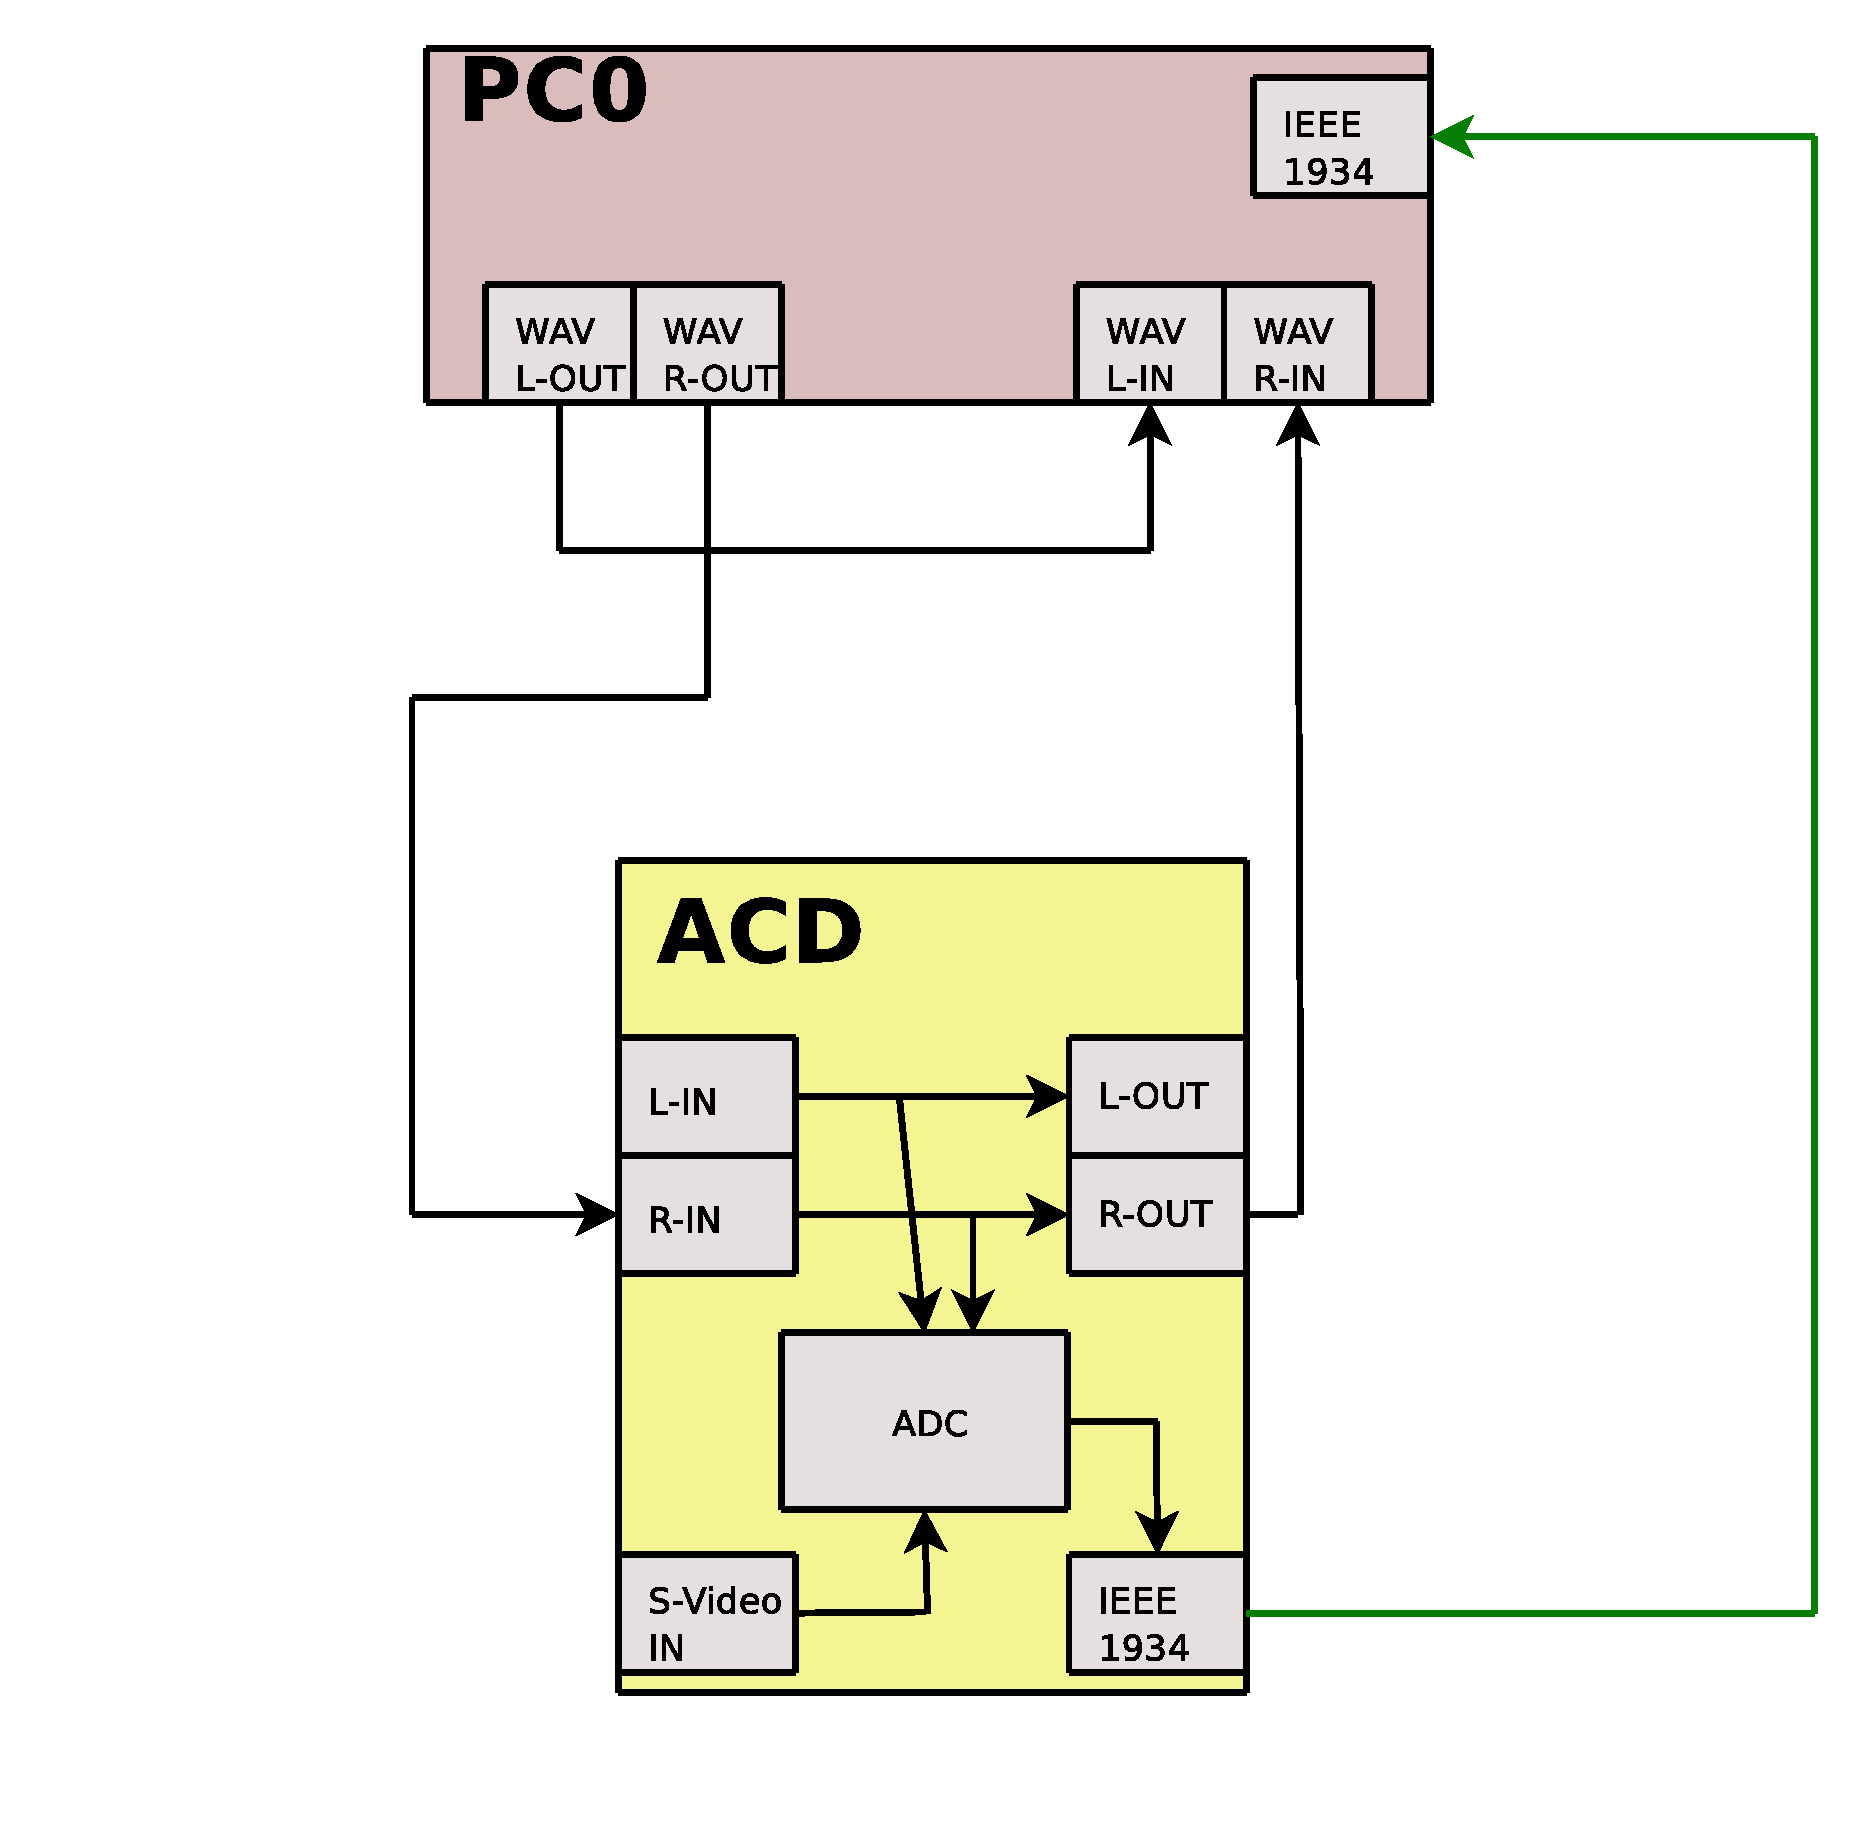
\includegraphics[width=0.32\textwidth]{include/linguometer/images/delay_schemaR.eps}}

	\subfigure[\label{fig:linguometer:architecture:sig:delay:1}]
	{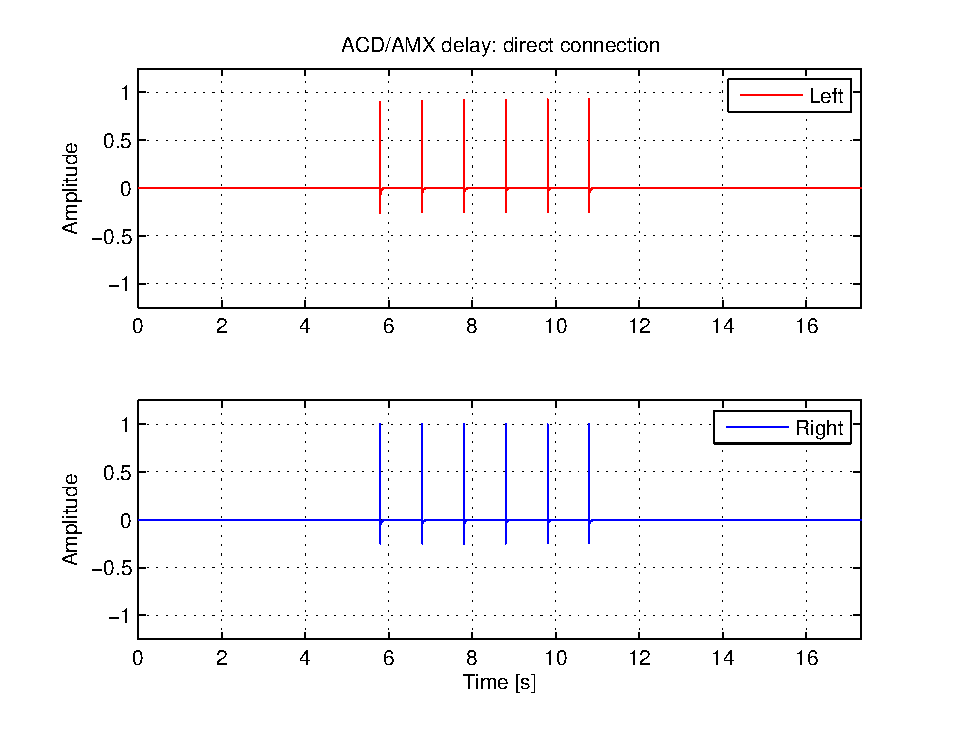
\includegraphics[width=0.32\textwidth]{include/linguometer/images/delay_fullT.eps}}
	\subfigure[\label{fig:linguometer:architecture:sig:delay:2}]
	{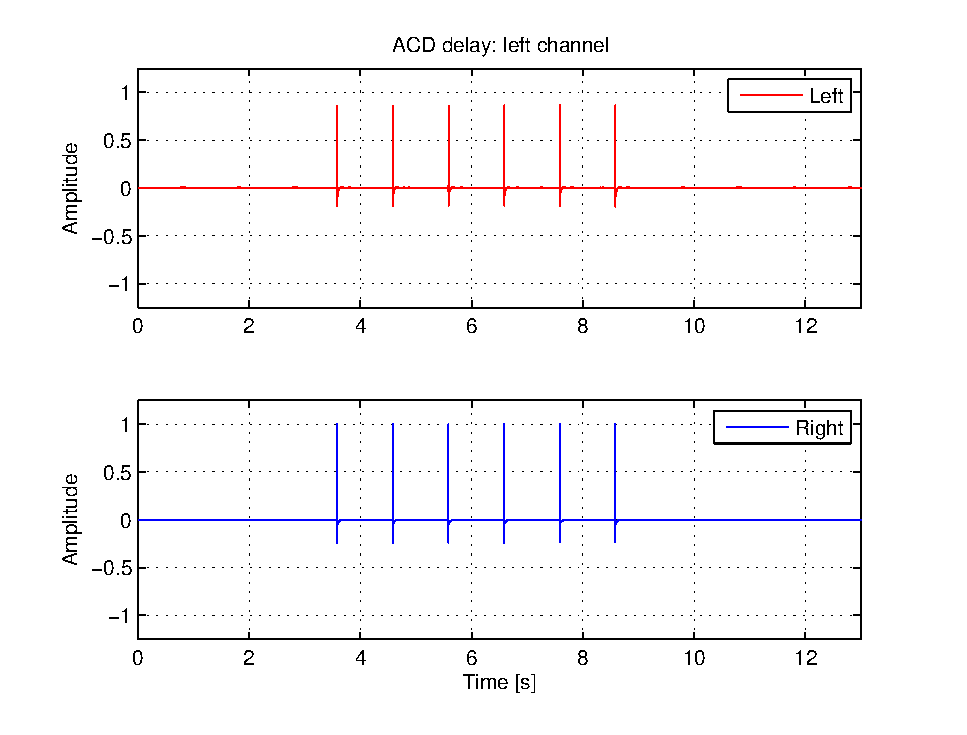
\includegraphics[width=0.32\textwidth]{include/linguometer/images/delay_fullL.eps}}
	\subfigure[\label{fig:linguometer:architecture:sig:delay:3}]
	{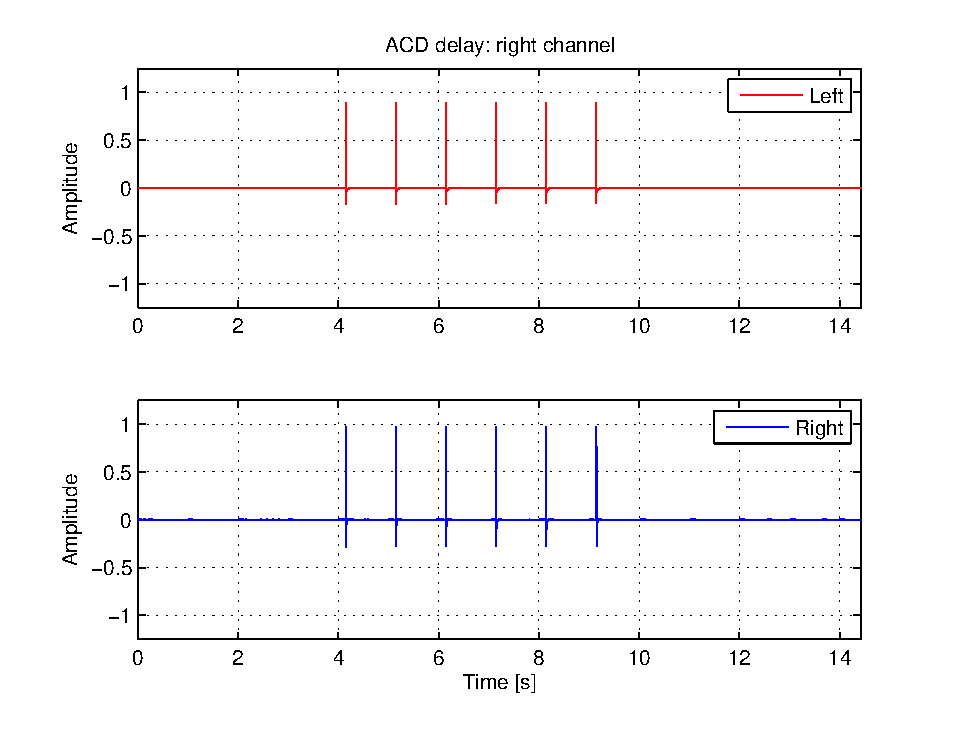
\includegraphics[width=0.32\textwidth]{include/linguometer/images/delay_fullR.eps}}
	
	\subfigure[\label{fig:linguometer:architecture:sig:delay:4}]
	{\includegraphics[width=0.32\textwidth]{include/linguometer/images/delay_zoomT.eps}}
	\subfigure[\label{fig:linguometer:architecture:sig:delay:5}]
	{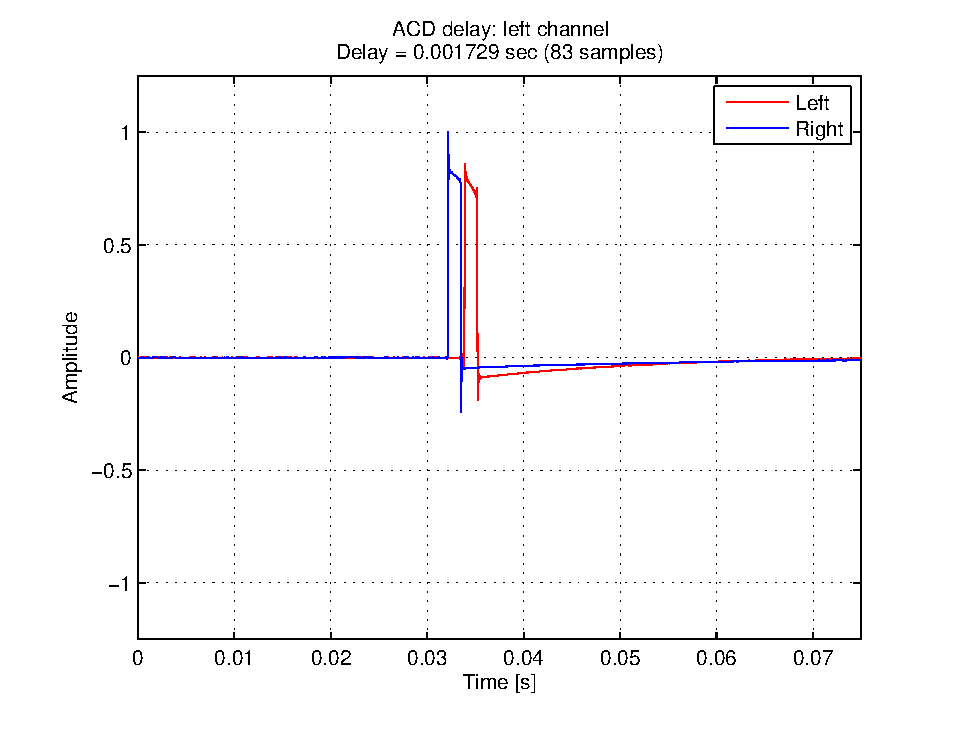
\includegraphics[width=0.32\textwidth]{include/linguometer/images/delay_zoomL.eps}}
	\subfigure[\label{fig:linguometer:architecture:sig:delay:6}]
	{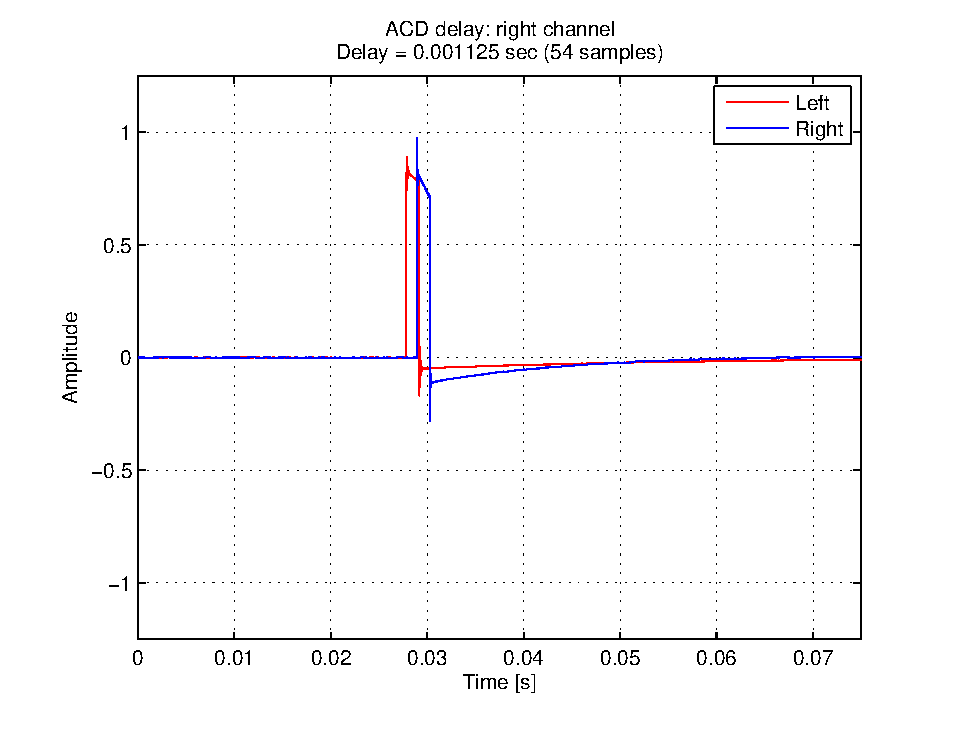
\includegraphics[width=0.32\textwidth]{include/linguometer/images/delay_zoomR.eps}}
	
	\caption[Acquisition card delay]{\textbf{Acquisition card delay}:
	(a) direct connection (reference test);
	(b) left channel through the delayed device;
	(c) right channel through the delayed device.
	(d, e, f) Test signals as they are acquired by \sig{PC0}.
	(g, h, i) First peak of the acquired signals.
	The plots refer to the first trial.
	}
	\label{fig:linguometer:architecture:sig:delay}
\end{figure}
% ---------------------------------------------------------------------------- %

The author measured the delays that affect the \sig{AMX} mixer
\sig{Line1 L-IN}/\sig{Mixer L-OUT} and the
\sig{Line1 R-IN}/\sig{Mixer R-OUT} connections.
Furthermore, the  \sig{ACD} acquisition card
\sig{L-IN}/\sig{L-OUT} and
\sig{R-IN}/\sig{R-OUT} delays have been measured.

In order to measure the delays, the setup control computer \sig{PC0} has been 
used.
A stereo audio signal with a total of six peaks has been built, 
following the same procedure used for the \emph{lmwords} segmentation signals
(PCM 16 bit, 48kHz).
The main idea behind the delay test is trivial. The test signal has got two
identical channels, each one with six peaks.
The digital signal is converted in its analog form by \sig{PC1}, simply using
its sound card (line level outputs).
One out of the two channels is routed trough the delay-affected device and then
back to \sig{PC1}, using the sound card line level inputs.
The remaining channel, used as reference, is routed directly
from the line level output connector to the line level input connector.
Being the original channels perfectly synchronized, if the measured device
introduce some kind of time shift in the signal, it should be detectable by the
means of cross-correlation.
Figure~\ref{fig:linguometer:architecture:sig:delay} shows the building blocks
and the resulting signals obtained measuring the acquisition card delay.

A total of five different tests have been executed, three times each.
In the first case, the test signal is routed directly from the line level output
to the line level input connector, as shown in
Figure~\ref{fig:linguometer:architecture:sig:delay:7}.
In the second and third cases,
Figures~\ref{fig:linguometer:architecture:sig:delay:8} and
and~\ref{fig:linguometer:architecture:sig:delay:9},
the \sig{ACD} \sig{L-IN}/\sig{L-OUT} and
the \sig{R-IN}/\sig{R-OUT} delays have been measured routing one audio channel
at the time (\sig{WAV L-OUT} and \sig{WAV R-OUT}) trough the delay affected
device (in this case, \sig{ACD}).
In the latest two cases, the \sig{AMX} \sig{Line1 L-IN}/\sig{Mixer L-OUT} and 
\sig{Line1 R-IN}/\sig{Mixer R-OUT} delays have been measured, following the same
procedure used to measure the \sig{ACD} delays.
%The left and the right channels of the test signal are identical. 
%In other words the peak appear at the same time in both the channels.
Figures~\ref{fig:linguometer:architecture:sig:delay:1}, 
\ref{fig:linguometer:architecture:sig:delay:2} and
\ref{fig:linguometer:architecture:sig:delay:3} show the test signal 
as recorded by the \sig{PC0} \sig{WAV L-IN}/\sig{WAV R-IN} line level input.\\
Figures~\ref{fig:linguometer:architecture:sig:delay:4}, 
\ref{fig:linguometer:architecture:sig:delay:5} and
\ref{fig:linguometer:architecture:sig:delay:6} show the
first peak of the recorded test signal.
\begin{table}[ht!]
  \begin{center}
  \begin{scriptsize}
	\begin{tabular}{|c|c|cc|cc|}
	  \hline
	   & \textbf{Direct} & \textbf{ACD L.} & \textbf{ACD R.} & \textbf{AMX L.} & \textbf{AMX R.}\\
	  \hline
	  \textbf{Trial 1} & 1 & 83 & 54 & 22 & 24\\
	  \textbf{Trial 2} & 1 & 82 & 52 & 22 & 22\\
	  \textbf{Trial 3} & 2 & 83 & 53 & 25 & 23\\
	  \hline
	  \textbf{AVG} & 1.33 & 82.67 & 53.00 & 23.00 & 23.00\\
	  \textbf{STD} & 0.58 & 0.58 & 1.00 & 1.73 & 1.00\\
	  \hline
	  \textbf{AVG} (ms) & 0.028 & 1.722 & 1.104 & 0.480 & 0.480\\
	  \textbf{STD} (ms) & 0.012 & 0.021 & 0.021 & 0.036 & 0.021\\
	  \hline
  \end{tabular}
  \end{scriptsize}
  \end{center}
	\caption[Acquisition card and mixer delays]{\textbf{Acquisition card and
	mixer delays}: the last two rows values are in milliseconds. Where not
	specified, values are in samples.}
 \label {tab:linguometer:architecture:sig:delay}
\end{table}


Table~\ref{tab:linguometer:architecture:sig:delay} shows the results of the
three trials. As expected, the direct connection test is not affected by a
significant delay. The delays affecting the right and the left acquisition card
channels are not constant, although they are constant in time. 
On the other hand, the delays affecting the audio mixer appear to be constant
both between the two channels and in time.
% ---------------------------------------------------------------------------- %
\subsection{Ultrasonograpic transducer: interference compensation}
\label{sec:linguometer:technical:interference}
% ---------------------------------------------------------------------------- %
As explained in the previous chapter, recording simultaneously with the
articulograph and the ultrasound system means placing the ultrasonograpic 
transducer inside the EMA-Cube frame of reference
(\S\ref{ch:linguometer:instrumentation:custom}).
In this context, the ultrasonograpic transducer could  
alter the physical properties of the electromagnetic field generated by the six
AG500 reference coils, thus invalidating the kinesthetic information acquired.
In this section, the compensation of the interference is discussed.

Before going any further with the dissertation, it is important to explicit what
the author means for inter-sensor distance (\emph{ISD}).
Three articulographic sensors are attached to a pair of glasses the subjects 
wear during the investigations.
Previously, it has been said that those sensors play a crucial role in
head-motion compensation.
In fact, the three glasses sensors acquire the kinesthetic information of head
movement.
Furthermore, those sensors are attached to a rigid body, that is the pair of
glasses. For this reason, the euclidean distance between any pair of sensors
should remain constant during the recording. The euclidean distance matches, in
this context, the term ISD.

Being the glasses a rigid body, the calculated ISDs should meet two
requirements.
Firstly the ISDs should remain constant during the nine acquired
sequences\footnote{As it discussed in the next Chapter, each experiment is made
up by a total of nine articulographic recordings, one for each batch of 
stimuli.}.
Lastly, the variance of the calculated ISDs should be qualitatively ``small''
and comparable between sequences.
If the calculated ISDs do not meet those requirements, it means that the 
simple calibration of the articulograph is not enough to compensate for the
interference generate by the ultrasonograpic transducer.
On the other hand, if the ISDs meet the two requirements, the interference is
successfully compensated by the means of calibration.

The author strongly believes that a better approach to the problem exists.
The ideal measurement of the interference generated by the ultrasonograpic
transducer could be done using an optical tracker and a wire-frame cube.
By attaching the 12 available sensors to the cube and measuring the position 
of the cube with respect to a reference frame (e.g.: any point on the  
EMA-Cube), the spatial distortion can be easily measured and even compensated by
inverting the coordinate transformation induced by the interference.
Since an electromagnetic tracker was not available, the author run many
different tests moving few sensors constraint to a rigid body inside the cube 
and evaluating the ISDs.
Although those tests are not presented in this thesis, the procedure has been 
embedded in the validation process the acquired data undergo before being
considered consistent.
Furthermore, the electronics that acquire the amplitude of one of the three 
sensors placed on the glasses proved to be faulty\footnote{If the sensor is
disconnected from the AG500 amplitude acquisition device, a current is still
seen by the diagnostic software. Furthermore, this amplitude does not remain
constant in time. In those conditions, the faulty sensor has been plugged to the
faulty port, but not being considered during analysis.}.
In order to determine if the interference compensation is consistent, the author
decided to measure the ISD between the two remaining sensors on the glasses and
between one of those and the sensor glued on the upper frontal teeth.\\

% ---------------------------------------------------------------------------- %
\begin{figure}
	\centering
	\subfigure[\label{fig:linguometer:technical:interference:ex:1}]
	{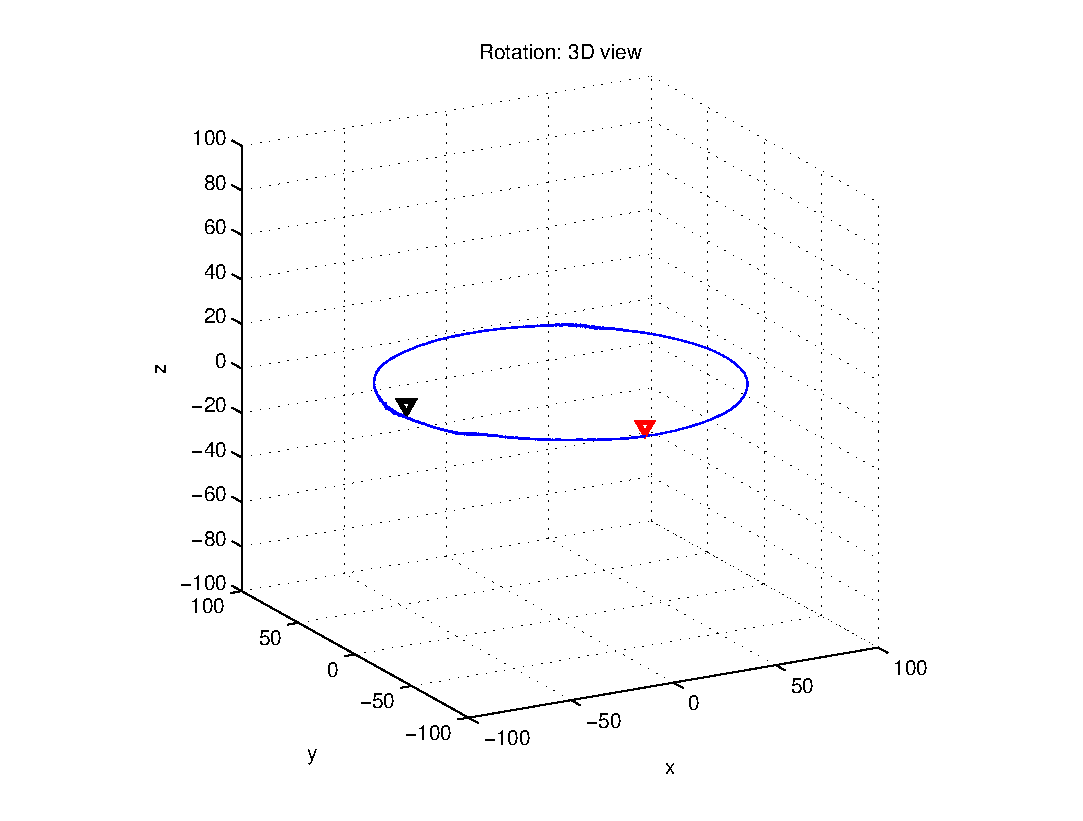
\includegraphics[width=0.45\textwidth]{include/linguometer/images/int_ex_1.eps}}
	\hspace{0.05\textwidth}
	\subfigure[\label{fig:linguometer:technical:interference:ex:2}]
	{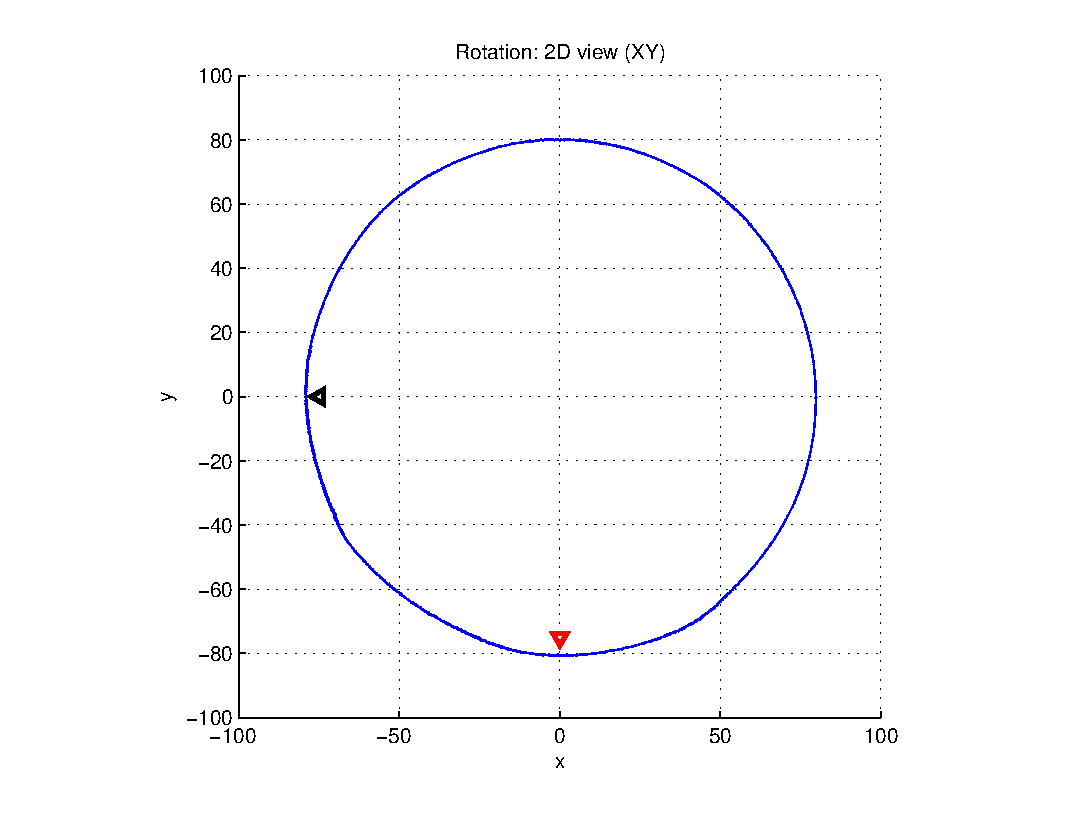
\includegraphics[width=0.45\textwidth]{include/linguometer/images/int_ex_2.eps}}
	
	\subfigure[\label{fig:linguometer:technical:interference:ex:3}]
	{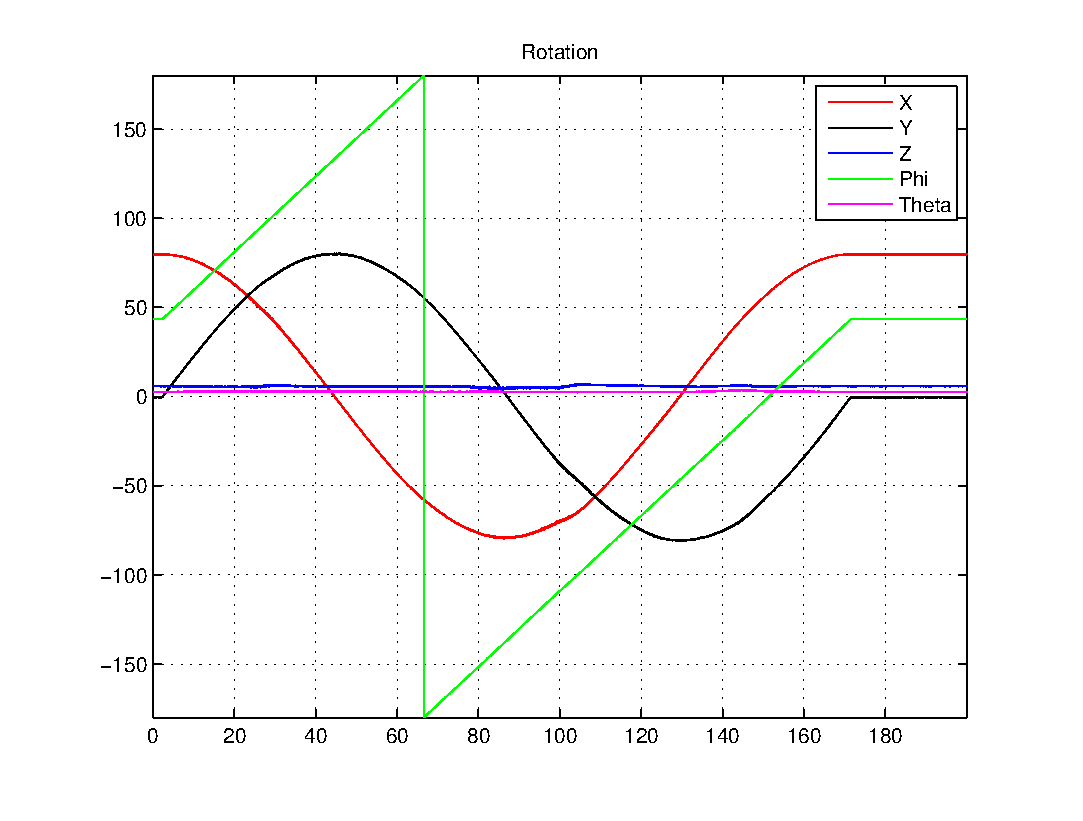
\includegraphics[width=0.45\textwidth]{include/linguometer/images/int_ex_3.eps}}
	\hspace{0.50\textwidth}
	
	\caption[Articulograph sensor rotation]{\textbf{Articulograph sensor
	rotation}: (a) tridimensional view of the rotation of a single sensor
	attached to the AG500 magazines used for calibration. 
	(b) Bidimensional projection (top view) of the previous plot.
	(c) This plot shows the 5DOF acquired by the means of electromagnetic 
	articulography. Three cartesian coordinates (X, Y and Z) and two spherical
	coordinates (azimuth Thetha and elevation Phi).
	Notes: the red triangle indicates the sensor starting point with respect
	to the XY plane (0 seconds). 
	The black triangle indicates the position of the ultrasonograpic 
	transducer (XY plane).
	The radius of the rotation measures 80 mm while the height at which 
	the rotation takes place measures 6.5 mm. The Theta angle measures circa
	5 $^{\circ}$ and the Phi angle varies during the rotation.
	}
	\label{fig:linguometer:technical:interference:ex}
\end{figure}
% ---------------------------------------------------------------------------- %

In this section, two different tests are presented. The first one is a
bidimensional test the author executed to verify the possibility of
recording  simultaneously with the articulograph and the ultrasound system.
While the first test has been executed one, the latter one has been executed for
each experiment and used for validating the acquired data.

Regarding the first test, three different cases are discussed.
In the first case, four articulograph sensors are calibrated without the 
ultrasonograpic transducer inside the frame of reference, thus
providing a reference condition since the articulograph is used in the best
possible conditions (e.g.: no electromagnetic interference).
The four sensors used for the investigation are left on the magazine used during
the calibration process, and the AG500 Circal is rotated by 360$^{\circ}$.
The amplitudes are acquired and the positions are computed as described in
\S\ref{sec:linguometer:instrumentation:ag}.
Figure~\ref{fig:linguometer:technical:interference:ex} provides an example
of the rotation of a sensor. Although this description is not strictly
necessary, it turns to be helpful to describe a problem that affects the 
articulograph AG500 algorithm used for the amplitude to position calculation.

% ---------------------------------------------------------------------------- %
\begin{figure}
	\centering
	\subfigure[\label{fig:linguometer:technical:interference:isd:1}]
	{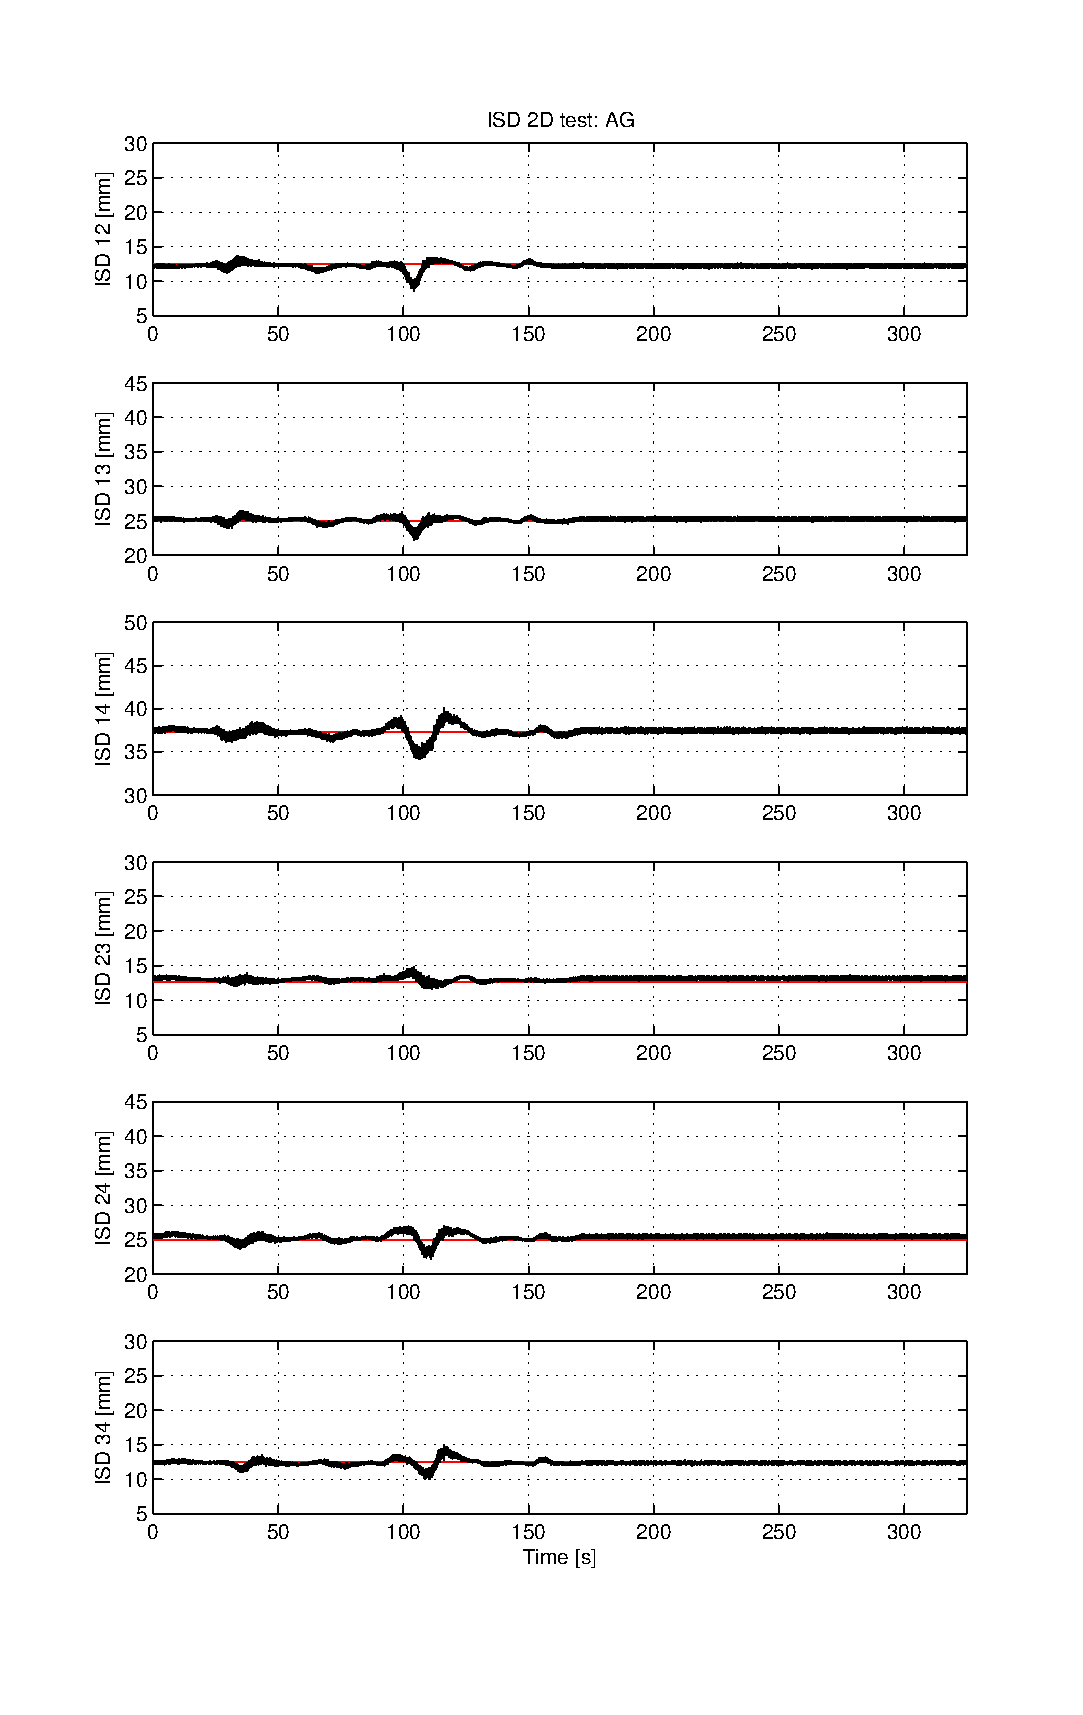
\includegraphics[width=0.35\textwidth]{include/linguometer/images/int_isd3d_1.eps}}
	\subfigure[\label{fig:linguometer:technical:interference:isd:2}]
	{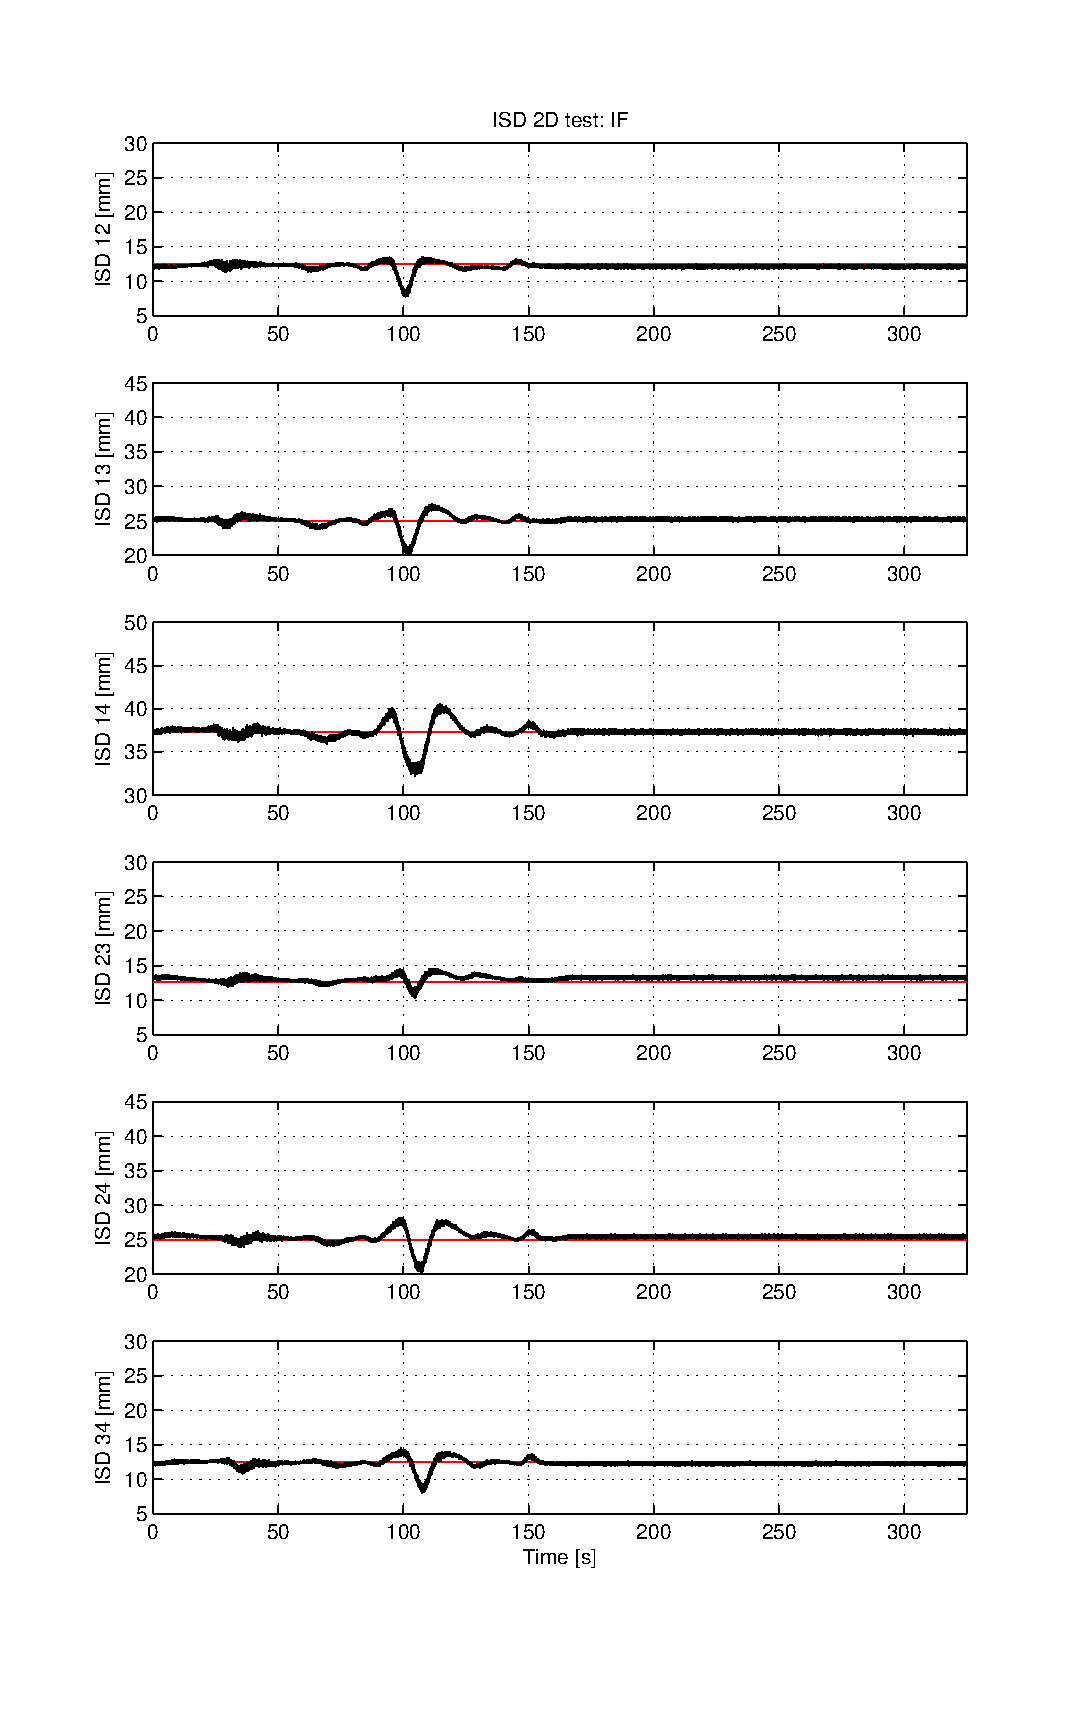
\includegraphics[width=0.35\textwidth]{include/linguometer/images/int_isd3d_2.eps}}

	\subfigure[\label{fig:linguometer:technical:interference:isd:3}]
	{\includegraphics[width=0.35\textwidth]{include/linguometer/images/int_isd3d_3.eps}}
	\hspace{0.35\textwidth}

	\caption[ISD results (ad-hoc test, XYZ)]{\textbf{ISD results (ad-hoc test, XYZ)}:
	ISDs calculated considering the three Cartesian coordinates of each 
	acquired sample (X, Y and Z).
	(a) AG test, (b) IF test and (c) LM test.
	Red plots: ISD between sensors 1 and 2. Black plots: ISD between sensors 2
	and 3. Blue plots: ISD between sensors 3 and 4. 
	Notes: ISD scale in millimiters, time scale in seconds. The revolution of
	the circal starts between 0 and 1.5 seconds and ends approximately at 170
	seconds. From 170 seconds to the end of the acquisition, the sensors remain
	still in the initial position.
	}
	\label{fig:linguometer:technical:interference:isd}
\end{figure}
% ---------------------------------------------------------------------------- %

In the second case, the ultrasonograpic transducer is placed inside the
EMA-Cube, and the sensors are rotated again as explained for the first case.
Finally, in the third case the articulograph is calibrated in the ``linguometer
configuration'', that is, with the ultrasonograpic transducer inside the
Ema-Cube.
As in the two preceding cases, a complete turn of the Circal is executed.

To sum up, three different cases are here presented. 
The first one deals with the articulograph in the best possible recording
conditions, that is without any interfering object inside the frame of 
reference (\emph{AG test}).
In the second case, the worst possible condition is created. In fact, the
ultrasonograpic probe is placed inside the frame of reference without an
appropriate calibration of the articulograph (\emph{IF test}).
This condition should reveal if some kind of interference exists by looking at
the ISD values.
If the interference can be compensated by the means of calibration, then the
third case should prove this hypothesis.

Figure~\ref{fig:linguometer:technical:interference:isd} shows the computed
ISDs for the three cases respectively.
At least for the first case (AG test), the ISD value should remain constant
along the whole rotation, but unfortunately this is not the case.
In fact, the ISD values remain constant only at the end of the rotation, when
the sensors are kept in a fixed position nearby the starting point
(e.g.: the red triangle in 
Figure~\ref{fig:linguometer:technical:interference:ex}).

% ---------------------------------------------------------------------------- %
\pagebreak
% ---------------------------------------------------------------------------- %
